\documentclass{beamer}

\usepackage[francais]{babel}

\usepackage{tikz}
\usepackage[compat=1.1.0]{tikz-feynman}
\usetikzlibrary{angles, quotes}
\usetikzlibrary{calc}
\usetikzlibrary{external}
\usetikzlibrary{decorations.pathreplacing, shapes.misc}
\usetikzlibrary{decorations.markings}
\tikzexternalize[prefix=tikz/]
\tikzset{external/system call={lualatex \tikzexternalcheckshellescape -halt-on-error -interaction=batchmode -jobname "\image" "\texsource"}}
\usepackage{shellesc}
\usepackage{subcaption}

\usepackage{geometry}
\usepackage{pgfplots}
\pgfplotsset{compat=1.17} 
\usepgfplotslibrary{fillbetween}
\usepackage{pgf-pie}

\usepackage{csquotes}
\usepackage{array}
\usepackage{multirow}
\usepackage[normalem]{ulem}
\usepackage{tabularx}
\usepackage{amsmath}
\usepackage{amssymb}
\usepackage{amsfonts}
\usepackage{physics}
\usepackage{graphicx}
\usepackage{xspace}


\usepackage[T1]{fontenc}
\UseRawInputEncoding
\usetheme{Warsaw}
\usepackage{pgfpages}
\usepackage{latexsym,xcolor,multicol,booktabs,calligra}
\usepackage{listings,stackengine}
\usepackage{subcaption}
\usepackage{caption}
\captionsetup[figure]{font=footnotesize}
\usepackage{tabularx}

\usepackage{QUT}
\usepackage{appendixnumberbeamer}

\usepackage{amsmath}
\usepackage{amssymb}
\usepackage{amsfonts}
\usepackage{mathtools}
\usepackage{physics}
\usepackage{graphicx}
\usepackage{dsfont}
\usepackage{xspace}

\definecolor{deepblue}{rgb}{0,0,0.5}
\definecolor{deepred}{rgb}{0.6,0,0}
\definecolor{deepgreen}{rgb}{0,0.5,0}
\definecolor{halfgray}{gray}{0.55}

\lstset{
    basicstyle=\ttfamily\small,
    keywordstyle=\bfseries\color{deepblue},
    emphstyle=\ttfamily\color{deepred},
    stringstyle=\color{deepgreen},
    numbers=left,
    numberstyle=\small\color{halfgray},
    rulesepcolor=\color{red!20!green!20!blue!20},
    frame=shadowbox,
}

\def\lemaitre{\textsc{Lemaître}\xspace}
\def\skysurvey{\texttt{skysurvey}\xspace}
\def\pets{\texttt{PETS}\xspace}
\def\nacl{\texttt{NaCl}\xspace}
\def\edris{\texttt{EDRIS}\xspace}
\def\saltd{\texttt{SALT2.4}\xspace}
\newcommand{\credits}[1]{\tiny Credits : #1}


\title[Mesure de la croissance des structures avec DESI et ZTF]{Mesure de la croissance des structures avec les galaxies du DESI BGS et les supernovae de type Ia de ZTF : vers une analyse jointe}
\subtitle{Stage de fin d'études au LPNHE}
\author[Antoine Gilles-{}-Lordet]{Antoine Gilles--Lordet \\ \footnotesize encadré par Pauline Zarrouk et Nicolas Regnault}
\date{10 octobre 2024}

\begin{document}

\frame{\titlepage}

\section{Introduction}

\subsection{Contexte}

\begin{frame}{Cosmologie}
\begin{columns}
\begin{column}{0.5\textwidth}
	\begin{itemize}
		\item 	Le modèle cosmologique basée sur la relativité générale le plus simple est $\Lambda$CDM
		\item Décrit remarquablement bien les données
		\item De nombreux programmes (Euclid, JWST, DESI, LSST...)...
		\item ...pour différentes sondes cosmologiques : CMB, lentillage gravitationnel faible, SNe Ia, galaxies
	\end{itemize}
\end{column}
\begin{column}{0.5\textwidth}
\begin{figure}
	\centering
	\resizebox{\textwidth}{!}{
	\begin{tikzpicture}
		\pie[explode=0.05,
			text=pin,
			radius=2,
			color={orange!60, purple!60, yellow!30}]
			{68.3/{\small Énergie Noire}, 26.5/{\small Matière Noire}, 4.9/{\small Matière ordinaire}}
	\end{tikzpicture}}
	\caption{Composition de l'Univers tel que décrit par $\Lambda$CDM}
\end{figure}
\end{column}
\end{columns}
\end{frame}

%\begin{frame}{Matière noire et galaxies}
%	La matière noire est nécessaire pour expliquer la vitesses de rotation des galaxies et la distribution de matière dans l'univers
%	\begin{figure}
%		\centering
%		\includegraphics[width=.7\textwidth]{figures/Rotation_curve_galaxy.png}
%		\caption{Courbe de rotation de la galaxie spirale Messier 33 \\ \credits{Wikipedia}}
%	\end{figure}
%\end{frame}

\begin{frame}{Energie noire}
\begin{columns}
\begin{column}{0.6\textwidth}
	\begin{itemize}
\item L'énergie noire a été introduite pour expliquer l'accélération de l'expansion de l'univers
\item	Cette accélération a été découverte à l'aide de SNe Ia par S. Perlmutter, B. Schmidt et A. Riess (Prix Nobel 2011)
\item Constante cosmologique $\Lambda$ ? Energie noire ? Modèle alternatif de gravité ?
\end{itemize}
\end{column}
\begin{column}{0.4\textwidth}
	\begin{figure}
		\centering
		\includegraphics[height=0.6\textheight]{figures/Perlmutter_Schmidt.png}
		\caption{Diagramme de Hubble construit par Perlmutter et Schmidt en 2003}
	\end{figure}
\end{column}
\end{columns}
\end{frame}

\begin{frame}{Supernovae de type Ia}
\begin{columns}
\begin{column}{.5\textwidth}
	\begin{figure}
		\centering
		\includegraphics[width=.8\textwidth, trim={0 12cm 0 0}, clip]{figures/SNe-Ia-stretch.jpg}
		\caption{SNe Ia avant normalisation du stretch $x_1$}
	\end{figure}
\end{column}
\begin{column}{.5\textwidth}
	\begin{figure}
		\centering
		\includegraphics[width=.8\textwidth, trim={0 0 0 12.5cm}, clip]{figures/SNe-Ia-stretch.jpg}
		\caption{SNe Ia après normalisation du stretch $x_1$}
	\end{figure}
\end{column}
\end{columns}
Les magnitudes des SNeIa sont décrites par la formule de Tripp
\begin{equation}
	M^*_{b,SN} = M_b - \alpha x_{1,SN} + \beta c_{SN} + n(\sigma_{int})
\end{equation}
\end{frame}

\subsection{Observations}

% Accentuer le côté impressionnant de la chose ! Données déjà prises, et encore en cours

\subsubsection{ZTF}
\begin{frame}{Zwicky Transient Facility}
% Déplacer les LC sur slides avec la footprint de ZTF seule, rajouter image globale des telescopes et focal plane size
\begin{itemize}
	\item Situé à l'Observatoire de Palomar, utilise le telescope P48
	\item 1,22m de diamètre pour un champ de 47 degrés carré
	\item 16 CCDs de $6144 \times 6160$ pixels
	\item Couvre le ciel de l'hémisphère nord deux fois par nuit
\end{itemize}
\begin{columns}
	\begin{column}{.55\textwidth}
	\begin{figure}
		\centering
		\resizebox{.95\textwidth}{!}{
		\begin{tikzpicture}
			\node[anchor=south west, inner sep=0] (ztf) at (0,0) {\includegraphics[width=\textwidth]{figures/ztf_palomar.jpg}};
			\begin{scope}[x={(ztf.south east)},y={(ztf.north west)}]
				\draw[red, line width=2pt] (0.16,0.62) circle (2mm);
			\end{scope}
		\end{tikzpicture}}
		\caption{Telescope P48 utilisé par ZTF \\ \credits{Caltech/Palomar}}
	\end{figure}
	\end{column}
	
	\begin{column}{.45\textwidth}
	\begin{figure}
		\centering
		\includegraphics[width=.95\textwidth]{figures/ztf-camera-fov.jpg}
		\caption{Comparaison à l'échelle des champs de plusieurs relevés \credits{Caltech/Palomar}}
	\end{figure}
	\end{column}
\end{columns}
\end{frame}

\begin{frame}{Observations des SNe Ia}
\begin{columns}
\begin{column}{.5\textwidth}
\begin{figure}
	\centering
	\includegraphics[width=\textwidth]{figures/ztf_on_dust.png}
	\caption{SNe Ia observées par ZTF sur fond de carte de poussières déterminée par Planck}
\end{figure}
\end{column}
\begin{column}{.5\textwidth}
\begin{figure}
	\centering
	\includegraphics[width=\textwidth, trim={1cm 1cm 1cm 2cm}, clip]{figures/ZTF_lightcurves.png}
	\caption{Exemples de courbes de lumière de SNe Ia \\ \credits{Caltech/Palomar}}
\end{figure}
\end{column}
\end{columns}
\end{frame}




\subsubsection{DESI}

\begin{frame}{Dark Energy Spectroscopic Instrument}
% Plus gros relevé de galaxie disponible avec un seul télescope, 5000 en 30 minutes, avant 1000 en 1h30
% 2 slides : Telescope et plan focal, puis observations
% 		\item Mesure des spectres pour déterminer la positions 3D
%		\item But : contraindre l'énergie noire
\begin{itemize}
	\item Utilise le Mayall Telescope à l'Observatoire de Kitt peak (USA)
	\item 4m de diamètre pour un champ de 8.0 degrés carré
	\item 5 000 fibres robotisées avec une pose de 30 minutes, au lieu de \\1 000 en 1h30
	\item $\sim 40$ millions de galaxies ciblées
	\item Prise de données débutée en 2021, pour 7 ans
\end{itemize}

\begin{columns}
\begin{column}{.5\textwidth}
	\begin{figure}
		\centering
		\includegraphics[width=0.75\textwidth]{figures/kitt_peak.png}
		\caption{Observatoire de Kitt Peak \\ \credits{University of California, Lawrence Berkeley National Laboratory}}
	\end{figure}
\end{column}
\begin{column}{.5\textwidth}
	\begin{figure}
		\centering
		\includegraphics[width=0.8\textwidth]{figures/DESI_robots.jpg}
		\caption{Plan focal du Mayall Telescope et zoom sur les robots\\ \credits{DESI Collaboration}}
	\end{figure}
\end{column}
\end{columns}
\end{frame}

\begin{frame}{Observations des galaxies}
\begin{columns}
\begin{column}{.5\textwidth}
	\begin{figure}
		\centering
	\includegraphics[width=\textwidth]{figures/desi_on_dust.png}
	\caption{Galaxies observées par DESI sur fond de carte de poussières déterminée par Planck}
	\end{figure}
\end{column}
\begin{column}{.5\textwidth}
	\begin{figure}
		\centering
		\includegraphics[width=0.8\textwidth]{figures/DESI_spec.png}
		\caption{Exemple de spectre mesuré par DESI\\ \credits{DESI Collaboration}}
	\end{figure}
\end{column}
\end{columns}
\end{frame}

\begin{frame}{Observations du même ciel}
\begin{figure}
	\centering
	\includegraphics[width=0.8\textwidth, trim={3mm 1cm 3mm 1cm}, clip]{figures/ztf_desi_on_dust.png}
	\caption{SNe Ia de ZTF et galaxies de DESI}
\end{figure}
\end{frame}

\subsection{Croissances des structures}

% montrer l'évolution des distances avec les rsd

\begin{frame}{Croissance des structures dans l'Univers}
\begin{columns}
\begin{column}{.4\textwidth}
\begin{itemize}
\item<1-> Taux de croissance des structure $f(z)$
\item<2-> Écart-type de densité dans une sphère de 8 Mpc \textcolor{deepgreen}{$\sigma_8(z)$}
\item<3> Paramètre composite $f\sigma_8$
\end{itemize}
\end{column}
\begin{column}{.6\textwidth}
	\begin{figure}
		\centering
		\begin{tikzpicture}
			\node[anchor=south west,inner sep=0] (image) at (0,0) {\includegraphics[width=0.8\textwidth]{figures/struct_growth.png}};
			\only<2-3>{
			\begin{scope}[x={(image.south east)},y={(image.north west)},
					    every node/.style={draw, circle, deepgreen, line width=2pt}]
				\node at (0.3,0.8) {};
				\node at (0.515,0.8) {};
				\node at (0.73,0.8) {};
				\node at (0.945,0.8) {};
			\end{scope}}
		\end{tikzpicture}
		\caption{Formation des structures pour différentes compositions de l'Univers\\ \credits{Kauffmann, Colberg, Diaferio, and White}}
	\end{figure}
\end{column}
\end{columns}
\end{frame}

\begin{frame}{Analyse des structures}
%	Les vitesses particulières des galaxies sont proportionnelles à $f(z) \sigma_8(z)$ et décalent le redshift observé
%	\begin{equation}
%		1+z_{obs} = (1+\textcolor{red}{z_{cosmo}}) (1 + \textcolor{blue}{z_{pec}}) = (1+\textcolor{red}{z_{cosmo}}) \qty(1 + \frac{1}{c} \textcolor{blue}{\vb v_{pec}} \cdot \vu r)
%	\end{equation}
\begin{columns}
	\begin{column}<1->[t]{.5\textwidth}
	Clustering des galaxies~:
	\begin{itemize}
		\item requiert de nombreuses galaxies
		\item peu performant à bas redshift
	\end{itemize}
	\begin{figure}
		\centering
		\resizebox{.9\textwidth}{!}{
		\begin{tikzpicture}
			\node[anchor=south west,inner sep=0] (tele) at (0,0.2) {\includegraphics[width=5mm]{figures/telescope_schema.png}};
			\node[anchor=south west, inner sep=0] (gal) at (3,2) {\includegraphics[width=1cm]{figures/Andromede.jpg}};
			\draw[dashed] (tele) -- (gal);
			\draw[-stealth, line width=3pt, red] (gal) -- ++(1.5,1) node[above left, pos=0.5] {$1+z_{cosmo}$};
			\draw[-stealth, line width=3pt, blue] (gal) -- ++(1,-.5) node[below, pos=0.5] {$v_{pec}$};
			\node[draw, ellipse, blue] at (6, 1) {Surdensité};
		\end{tikzpicture}}
		\caption{Distortion des redshifts due aux vitesses particulières}
	\end{figure}
	\end{column}
	\begin{column}<2>[t]{.5\textwidth}
	Nouvelle sonde à bas redshift, les SNe Ia
	\begin{itemize}
		\item particulièrement performant à bas redshift
	\end{itemize}
	\begin{figure}
		\centering
		\includegraphics[width=\textwidth]{figures/Residues.png}
		\caption{Effets des vitesses particulières pour les SNe Ia\\ \credits{B. Carreres}}
	\end{figure}
	\end{column}
\end{columns}
\end{frame}

		
\begin{frame}{Analyse jointe entre galaxies et SNe Ia}
\begin{figure}
	\centering
	\only<1-3>{%
	\begin{tikzpicture}
		\only<1>{\node[anchor=south west] (image1) at (0,0) {\includegraphics[width=.7\textwidth, trim={4cm, 3cm, 2cm, 3cm}, clip, page=12]{figures/Bautista_desi_ztf_growth.pdf}};}
		\only<2>{\node[anchor=south west] (image2) at (0,0) {\includegraphics[width=.7\textwidth, trim={4cm, 3cm, 2cm, 3cm}, clip, page=13]{figures/Bautista_desi_ztf_growth.pdf}};}
		\only<3>{\node[anchor=south west] (image3) at (0,0) {\includegraphics[width=.7\textwidth, trim={4cm, 3cm, 2cm, 3cm}, clip, page=14]{figures/Bautista_desi_ztf_growth.pdf}};
			\begin{scope}[x={(image3.south east)},y={(image3.north west)}]
				\draw[draw=none, fill=white] (0.27, 0.15) rectangle  ++(.1,.09);
				\draw[draw=none, fill=white] (0.26, 0.19) rectangle  ++(.05,.05);
			\end{scope}}
	\end{tikzpicture}%
	}%
	\caption{Gain apporté par les vitesses particulières des SNe sur $f\sigma_8$ \\ \credits{J. Bautista}}
\end{figure}
\end{frame}


\begin{frame}{Objectifs du stage}
\begin{itemize}
\item<1-> Reconstruire les vitesses particulières des SNe Ia en vue d'une analyse jointe avec les galaxies de DESI\\[2em]
\item<2-> Nécessite un nouveau pipeline d'analyse des SNe Ia de ZTF capable de traiter les volumes de données\\[2em]
\end{itemize}
\begin{block}<3>{Mon travail}
Mon travail : générer des simulations de supernovae en incluant les effets des vitesses particulières de DESI et les analyser pour reconstruire leurs vitesses particulières
\end{block}
\end{frame}

\section{Chaîne d'analyse cosmologique avec SNe Ia}

\begin{frame}{Plan de travail}
% Remettre LEMAITRE à chaque slide, avec l'avancée dans chaque module.
% Chaîne simplifiée SALT complète, puis montrer les nouveaux blocs. utilise un vieux modèle, statistique faible -> utiliser LEMAITRE
% retirer la calib, mettre la simu skysurvey en haut et dérouler la chaîne sur 3 slides
\begin{figure}
	\centering
	\only<1-3>{
		\resizebox{!}{0.8\textheight}{
		\begin{tikzpicture}[-stealth, line width=1.2pt]
			\node[rectangle, draw, red!50!black] (skys) at (0,0) {\skysurvey};
			\node[rectangle, draw, above right=of skys, color=blue, align=center] (uchuu) {INPUT \\ Simulation Uchuu};
			\node[rectangle, draw, left=of uchuu, color=blue, align=center] (logs) {INPUT \\ Logs d'observation de ZTF};

			\draw[black] (logs) edge (skys);
			\draw[orange] (uchuu) -- (skys);
			
			\uncover<2->{
			\node[rectangle, draw, below=of skys] (pets) {\pets};
			\node[rectangle, draw, below=of pets] (nacl) {\nacl};
			\node[rectangle, draw, below=of nacl] (edris) {\edris};
			\node[rectangle, draw, below=of edris,  align=center, color=green!70!black] (out) {Output \\ - $\mu_{obs}$ \\ - Cosmologie};
			\node[rectangle, draw, below= of out, color=green!70!black] (vpec) {$v_{pec}$};
			\draw[black] (skys) edge (pets) (pets) edge (nacl) (nacl) edge (edris) (edris) edge (out);
			\draw[dashed, orange] (skys) edge (pets) (pets) edge (nacl) (nacl) edge (edris) (edris) edge (out);
			\draw[orange] (out) -- (vpec);}

			\uncover<3>{
			\path (pets) -- (nacl) node[pos=.5] (mid) {};
			\node[rectangle, draw, right=of mid, align=center, red!50!black] (rec) {Reconstruction \\ avec \skysurvey};
			\draw[orange] (skys) -| (rec);
			\draw[orange] (rec) |- (edris);}
		\end{tikzpicture}
		}%
	}%
\end{figure}

%\begin{column}{.4\textwidth}
%Premiere intégration de la chaîne \lemaitre
%	\begin{itemize}
%	\item \pets~: Sélection des SNe
%	\item \nacl~: Entraînement d'un modèle de SNe Ia et ajustement des paramètres de standardisation
%	\item \edris~: Ajustement d'un modèle cosmologique
%	\end{itemize}
%\end{column}
\end{frame}
% Suivre la reconstruction d'une SNe

\subsection{Chaîne simplifiée avec \saltd}

\subsubsection{Générations des SNe}
% Observations (LC et spectres)

\begin{frame}{Générations des SNe avec \skysurvey~: observables}
\begin{figure}
	\centering
	\includegraphics[width=.9\textwidth]{figures/exemple_lc_sp.png}
	\caption{Exemple de courbes de lumière et de spectre pour une SNe Ia observée par ZTF\\ \credits{Mon Not R Astron Soc, Volume 510, Issue 2, February 2022, Pages 2228–2241}}
\end{figure}
\end{frame}

% Modèle pour les obtenir -> paramètres

\begin{frame}{Générations des SNe avec \skysurvey~: modèle \saltd}
\begin{itemize}
	\item Le modèle \saltd est décrit par la surface spectrale
	\begin{equation}
	    F(p, \lambda) = \textcolor{blue}{x_0} \times \qty[\textcolor{deepgreen}{M_0(p, \lambda)} + \textcolor{blue}{x_1} \textcolor{deepgreen}{M_1(p, \lambda)}] \times \exp[\textcolor{blue}{c}\ \textcolor{deepgreen}{CL(\lambda)}]
	\end{equation}
	\item 4 paramètres par SNe Ia $(x_0, x_1, c, t_{max})$
\end{itemize}

\begin{columns}
	\begin{column}{.5\textwidth}
		\begin{figure}
			\centering
			\includegraphics[width=.9\textwidth, trim={1cm 1cm 1cm 2cm}, clip]{figures/model_w_spectra.png}
			\caption{Surface spectrale et spectre à une phase donnée}
		\end{figure}
	\end{column}
	\begin{column}{.5\textwidth}
		\begin{figure}
			\centering
			\includegraphics[width=.9\textwidth, trim={1cm 1cm 1cm 2cm}, clip]{figures/model_w_lc.png}
			\caption{Surface spectrale et courbe de lumière à travers un filtre}
		\end{figure}
	\end{column}
\end{columns}
\end{frame}

% Distributions des paramètres de standardisations
\begin{frame}{Générations des SNe avec \skysurvey~: tirage des paramètres de standardisation}
\begin{columns}
\begin{column}[c]{.2\textwidth}
	\resizebox{\textwidth}{!}{
	\begin{tikzpicture}[-stealth, line width=1.2pt]
		\node[rectangle, draw, red, line width=3pt] (skys) at (0,0) {\skysurvey};
		\node[rectangle, draw, above right=of skys, color=blue, align=center] (uchuu) {Input \\ Simulation Uchuu};
		\node[rectangle, draw, left=of uchuu, color=blue, align=center] (logs) {Input \\ Logs d'observation de ZTF};
		\draw[black] (logs) edge (skys);
		\draw[orange] (uchuu) edge(skys);
		
		\node[rectangle, draw, below=of skys] (pets) {\pets};
		\node[rectangle, draw, below=of pets] (nacl) {\nacl};
		\node[rectangle, draw, below=of nacl] (edris) {\edris};
		\node[rectangle, draw, below=of edris,  align=center, color=green!70!black] (out) {Output \\ - $\mu_{obs}$ \\ - Cosmologie};
		\node[rectangle, draw, below= of out, color=green!70!black] (vpec) {$v_{pec}$};
		\draw[black] (skys) edge (pets) (pets) edge (nacl) (nacl) edge (edris) (edris) edge (out);
		\draw[dashed, orange] (skys) edge (pets) (pets) edge (nacl) (nacl) edge (edris) (edris) edge (out);
		\draw[orange] (out) -- (vpec);

		\path (pets) -- (nacl) node[pos=.5] (mid) {};
		\node[rectangle, draw, right=of mid, align=center, red!50!black] (rec) {Reconstruction \\ avec \skysurvey \\ (\saltd)};
		\draw[orange] (skys) -| (rec);
		\draw[orange] (rec) |- (edris);
	\end{tikzpicture}}%
\end{column}
\begin{column}[c]{.8\textwidth}
\begin{figure}
	\centering
	\includegraphics[height=.6\textheight]{figures/SNe_sampling.png}
	\caption{Distribution des paramètres de standardisations}
\end{figure}
\end{column}
\end{columns}
\end{frame}

% Positions des SNe, redshift
\begin{frame}{Générations des SNe avec \skysurvey~: tirage des positions}
\begin{columns}
\begin{column}[c]{.2\textwidth}
\only<1-2>{
	\resizebox{\textwidth}{!}{
	\begin{tikzpicture}[-stealth, line width=1.2pt]
		\node[rectangle, draw, red, line width=3pt] (skys) at (0,0) {\skysurvey};
		\only<1>{\node[rectangle, draw, above right=of skys, blue, align=center] (uchuu) {Input \\ Simulation Uchuu};}
		\only<2>{\node[rectangle, draw, above right=of skys, red, line width=3pt, align=center] (uchuu) {Input \\ Simulation Uchuu};}

		\node[rectangle, draw, left=of uchuu, color=blue, align=center] (logs) {Input \\ Logs d'observation de ZTF};
		\draw[black] (logs) edge (skys);
		\only<1>{\draw[orange] (uchuu) edge(skys);}
		\only<2>{\draw[red, line width=3pt] (uchuu) edge(skys);}
		
		\node[rectangle, draw, below=of skys] (pets) {\pets};
		\node[rectangle, draw, below=of pets] (nacl) {\nacl};
		\node[rectangle, draw, below=of nacl] (edris) {\edris};
		\node[rectangle, draw, below=of edris,  align=center, color=green!70!black] (out) {Output \\ - $\mu_{obs}$ \\ - Cosmologie};
		\node[rectangle, draw, below= of out, color=green!70!black] (vpec) {$v_{pec}$};
		\draw[black] (skys) edge (pets) (pets) edge (nacl) (nacl) edge (edris) (edris) edge (out);
		\draw[dashed, orange] (skys) edge (pets) (pets) edge (nacl) (nacl) edge (edris) (edris) edge (out);
		\draw[orange] (out) -- (vpec);

		\path (pets) -- (nacl) node[pos=.5] (mid) {};
		\node[rectangle, draw, right=of mid, align=center, red!50!black] (rec) {Reconstruction \\ avec \skysurvey \\ (\saltd)};
		\draw[orange] (skys) -| (rec);
		\draw[orange] (rec) |- (edris);
	\end{tikzpicture}}%
	}
\end{column}
\begin{column}[c]{.8\textwidth}
\alt<2>{
\begin{figure}
	\centering
	\includegraphics[width=.45\textwidth]{figures/angular_draw.png}
	\hfill
	\includegraphics[width=.45\textwidth]{figures/redshift_draw.png}
	\caption{Distributions angulaires et en redshift des SNe Ia tirées à partir du catalogue Uchuu}
\end{figure}}{
\begin{figure}
	\centering
	\includegraphics[width=.45\textwidth]{figures/unif_angular_draw.png}
	\hfill
	\includegraphics[width=.45\textwidth]{figures/unif_redshift_draw.png}
	\caption{Distributions angulaire et des redshifts par défaut dans \skysurvey}
\end{figure}}
\end{column}
\end{columns}
\end{frame}


\begin{frame}{Courbes de lumière et spectres}
\begin{columns}
\begin{column}{.2\textwidth}
	\resizebox{\textwidth}{!}{
	\begin{tikzpicture}[-stealth, line width=1.2pt]
		\node[rectangle, draw, red, line width=3pt] (skys) at (0,0) {\skysurvey};
		\node[rectangle, draw, above right=of skys, blue, align=center] (uchuu) {Input \\ Simulation Uchuu};
		\node[rectangle, draw, left=of uchuu, red, line width=3pt, align=center] (logs) {Input \\ Logs d'observation de ZTF};
		\draw[red, line width=3pt] (logs) edge (skys);
		\draw[orange] (uchuu) edge(skys);
		
		\node[rectangle, draw, below=of skys] (pets) {\pets};
		\node[rectangle, draw, below=of pets] (nacl) {\nacl};
		\node[rectangle, draw, below=of nacl] (edris) {\edris};
		\node[rectangle, draw, below=of edris,  align=center, color=green!70!black] (out) {Output \\ - $\mu_{obs}$ \\ - Cosmologie};
		\node[rectangle, draw, below= of out, color=green!70!black] (vpec) {$v_{pec}$};
		\draw[black] (skys) edge (pets) (pets) edge (nacl) (nacl) edge (edris) (edris) edge (out);
		\draw[dashed, orange] (skys) edge (pets) (pets) edge (nacl) (nacl) edge (edris) (edris) edge (out);
		\draw[orange] (out) -- (vpec);

		\path (pets) -- (nacl) node[pos=.5] (mid) {};
		\node[rectangle, draw, right=of mid, align=center, red!50!black] (rec) {Reconstruction \\ avec \skysurvey \\ (\saltd)};
		\draw[orange] (skys) -| (rec);
		\draw[orange] (rec) |- (edris);
	\end{tikzpicture}}%
\end{column}

\begin{column}{.8\textwidth}
\begin{figure}
	\centering
	\includegraphics[width=.49\textwidth]{figures/26_lc.png}
	\hfill
	\includegraphics[width=.49\textwidth]{figures/26_spec.png}
	\caption{Courbes de lumière et spectre simulés pour une SNe Ia}
\end{figure}
	\end{column}
\end{columns}
\end{frame}


\subsubsection{Paramètres de standardisations avec \saltd}

\begin{frame}{Reconstruction avec \saltd}
\begin{columns}
	\begin{column}{.2\textwidth}
	\resizebox{\textwidth}{!}{
	\begin{tikzpicture}[-stealth, line width=1.2pt]
		\node[rectangle, draw, red, red!50!black] (skys) at (0,0) {\skysurvey};
		\node[rectangle, draw, above right=of skys, blue, align=center] (uchuu) {Input \\ Simulation Uchuu};
		\node[rectangle, draw, left=of uchuu, blue, align=center] (logs) {Input \\ Logs d'observation de ZTF};
		\draw[black] (logs) edge (skys);
		\draw[orange] (uchuu) edge(skys);
		
		\node[rectangle, draw, below=of skys] (pets) {\pets};
		\node[rectangle, draw, below=of pets] (nacl) {\nacl};
		\node[rectangle, draw, below=of nacl] (edris) {\edris};
		\node[rectangle, draw, below=of edris,  align=center, color=green!70!black] (out) {Output \\ - $\mu_{obs}$ \\ - Cosmologie};
		\node[rectangle, draw, below= of out, color=green!70!black] (vpec) {$v_{pec}$};
		\draw[black] (skys) edge (pets) (pets) edge (nacl) (nacl) edge (edris) (edris) edge (out);
		\draw[dashed, orange] (skys) edge (pets) (pets) edge (nacl) (nacl) edge (edris) (edris) edge (out);
		\draw[orange] (out) -- (vpec);

		\path (pets) -- (nacl) node[pos=.5] (mid) {};
		\node[rectangle, draw, right=of mid, align=center, red, line width=3pt] (rec) {Reconstruction \\ avec \skysurvey \\ (\saltd)};
		\draw[red, line width=3pt] (skys) -| (rec);
		\draw[red, line width=3pt] (rec) |- (edris);
	\end{tikzpicture}}%
	\end{column}
\begin{column}{.8\textwidth}
\begin{itemize}
\item<1-> Réutiliser le modèle \saltd pour reconstruire les paramètres de standardisations
\item<2> Puis obtenir les modules de distances à l'aide de la formule
\begin{equation}
	\mu_{SN} = -2.5\log_{10} x_{0,SN} + \alpha x_{1,SN} - \beta c_{SN}
\end{equation}
\end{itemize}
\end{column}
\end{columns}
\end{frame}

\begin{frame}{Paramètres de standardisation \saltd}
\begin{columns}
	\begin{column}{.2\textwidth}
	\resizebox{\textwidth}{!}{
	\begin{tikzpicture}[-stealth, line width=1.2pt]
		\node[rectangle, draw, red, red!50!black] (skys) at (0,0) {\skysurvey};
		\node[rectangle, draw, above right=of skys, blue, align=center] (uchuu) {Input \\ Simulation Uchuu};
		\node[rectangle, draw, left=of uchuu, blue, align=center] (logs) {Input \\ Logs d'observation de ZTF};
		\draw[black] (logs) edge (skys);
		\draw[orange] (uchuu) edge(skys);
		
		\node[rectangle, draw, below=of skys] (pets) {\pets};
		\node[rectangle, draw, below=of pets] (nacl) {\nacl};
		\node[rectangle, draw, below=of nacl] (edris) {\edris};
		\node[rectangle, draw, below=of edris,  align=center, color=green!70!black] (out) {Output \\ - $\mu_{obs}$ \\ - Cosmologie};
		\node[rectangle, draw, below= of out, color=green!70!black] (vpec) {$v_{pec}$};
		\draw[black] (skys) edge (pets) (pets) edge (nacl) (nacl) edge (edris) (edris) edge (out);
		\draw[dashed, orange] (skys) edge (pets) (pets) edge (nacl) (nacl) edge (edris) (edris) edge (out);
		\draw[orange] (out) -- (vpec);

		\path (pets) -- (nacl) node[pos=.5] (mid) {};
		\node[rectangle, draw, right=of mid, align=center, red, line width=3pt] (rec) {Reconstruction \\ avec \skysurvey \\ (\saltd)};
		\draw[red, line width=3pt] (skys) -| (rec);
		\draw[red, line width=3pt] (rec) |- (edris);
	\end{tikzpicture}}%
	\end{column}
\begin{column}{.8\textwidth}
\begin{figure}
	\begin{subfigure}{0.49\textwidth}
		\centering
		\includegraphics[width=.7\textwidth]{figures/salt_x0_new.png}
		\includegraphics[width=.7\textwidth]{figures/salt_c_new.png}
	\end{subfigure}
	\begin{subfigure}{0.49\textwidth}
		\centering
		\includegraphics[width=.7\textwidth]{figures/salt_x1_new.png}
		\includegraphics[width=.7\textwidth]{figures/salt_tmax_new.png}
	\end{subfigure}
	\caption{Paramètres de standardisations reconstruits avec \saltd}
\end{figure}
\end{column}
\end{columns}
\end{frame}

\begin{frame}{Modules de distance \saltd}
\begin{columns}
	\begin{column}{.2\textwidth}
	\resizebox{\textwidth}{!}{
	\begin{tikzpicture}[-stealth, line width=1.2pt]
		\node[rectangle, draw, red, red!50!black] (skys) at (0,0) {\skysurvey};
		\node[rectangle, draw, above right=of skys, blue, align=center] (uchuu) {Input \\ Simulation Uchuu};
		\node[rectangle, draw, left=of uchuu, blue, align=center] (logs) {Input \\ Logs d'observation de ZTF};
		\draw[black] (logs) edge (skys);
		\draw[orange] (uchuu) edge(skys);
		
		\node[rectangle, draw, below=of skys] (pets) {\pets};
		\node[rectangle, draw, below=of pets] (nacl) {\nacl};
		\node[rectangle, draw, below=of nacl] (edris) {\edris};
		\node[rectangle, draw, below=of edris,  align=center, color=green!70!black] (out) {Output \\ - $\mu_{obs}$ \\ - Cosmologie};
		\node[rectangle, draw, below= of out, color=green!70!black] (vpec) {$v_{pec}$};
		\draw[black] (skys) edge (pets) (pets) edge (nacl) (nacl) edge (edris) (edris) edge (out);
		\draw[dashed, orange] (skys) edge (pets) (pets) edge (nacl) (nacl) edge (edris) (edris) edge (out);
		\draw[orange] (out) -- (vpec);

		\path (pets) -- (nacl) node[pos=.5] (mid) {};
		\node[rectangle, draw, right=of mid, align=center, red, line width=3pt] (rec) {Reconstruction \\ avec \skysurvey \\ (\saltd)};
		\draw[red, line width=3pt] (skys) -| (rec);
		\draw[red, line width=3pt] (rec) |- (edris);
	\end{tikzpicture}}%
	\end{column}
\begin{column}{.8\textwidth}
\begin{figure}
	\centering
	\includegraphics[height=.7\textheight]{figures/salt_mu_new.png}
	\caption{Modules de distance avec \saltd}
\end{figure}
\end{column}
\end{columns}
\end{frame}

\subsubsection{Cosmologie reconstruite avec \edris}

% RETIRER SNLS et les mesures de la légende

\begin{frame}{Modules de distance et cosmologie reconstruits par \edris}
\begin{columns}
	\begin{column}{.2\textwidth}
	\resizebox{\textwidth}{!}{
	\begin{tikzpicture}[-stealth, line width=1.2pt]
		\node[rectangle, draw, red, red!50!black] (skys) at (0,0) {\skysurvey};
		\node[rectangle, draw, above right=of skys, blue, align=center] (uchuu) {Input \\ Simulation Uchuu};
		\node[rectangle, draw, left=of uchuu, blue, align=center] (logs) {Input \\ Logs d'observation de ZTF};
		\draw[black] (logs) edge (skys);
		\draw[orange] (uchuu) edge(skys);
		
		\node[rectangle, draw, below=of skys] (pets) {\pets};
		\node[rectangle, draw, below=of pets] (nacl) {\nacl};
		\node[rectangle, draw, below=of nacl, red] (edris) {\edris};
		\node[rectangle, draw, below=of edris,  align=center, color=green!70!black] (out) {Output \\ - $\mu_{obs}$ \\ - Cosmologie};
		\node[rectangle, draw, below= of out, color=green!70!black] (vpec) {$v_{pec}$};
		\draw[black] (skys) edge (pets) (pets) edge (nacl) (nacl) edge (edris) (edris) edge (out);
		\draw[dashed, orange] (skys) edge (pets) (pets) edge (nacl) (nacl) edge (edris);
		\draw[red] (edris) edge (out);
		\draw[orange] (out) -- (vpec);

		\path (pets) -- (nacl) node[pos=.5] (mid) {};
		\node[rectangle, draw, right=of mid, align=center, red!50!black] (rec) {Reconstruction \\ avec \skysurvey \\ (\saltd)};
		\draw[orange] (skys) -| (rec);
		\draw[orange] (rec) |- (edris);
	\end{tikzpicture}}%
	\end{column}
	\begin{column}{.8\textwidth}
	\begin{figure}
		\centering
		\includegraphics[width=.8\textwidth]{figures/salt_cosmo.png}
		\caption{Cosmologie ajustée par \edris pour les résultats \saltd}
	\end{figure}
\end{column}
\end{columns}
\end{frame}

\subsubsection{Vitesses particulières}
\begin{frame}{Vitesses particulières}
Interpolation de la cosmologie $\mu(z)$ trouvée par \edris pour obtenir $z(\mu)$, puis récupération des vitesses particulières par
\begin{equation}
	v_{pec} = c(z_{obs} - z(\mu))
\end{equation}
\begin{figure}
	\centering
	\includegraphics[width=.48\textwidth]{figures/z_mu.png}
	\caption{Inversion de $\mu(z)$ en $z(\mu)$}
\end{figure}
\end{frame}

% Mettre la distribution des VP, sortir les data des encadrés.

\begin{frame}{Vitesses particulières reconstruites}
\begin{itemize}
\item Erreur moyenne~: $\overline{\Delta v_{pec, \saltd}} = -269.9$km.s$^{-1}$
\item Dispersion des erreurs~: $\sigma(\Delta v_{pec, \saltd}) = 791.9$km.s$^{-1}$
\item Dispersion théorique des erreurs due à la dispersion intrinsèque~: $\sigma(v_{pec, \saltd}, \sigma_{int}) = 581.5$km.s$^{-1}$
\end{itemize}
\begin{figure}
	\centering
	\includegraphics[width=.8\textwidth]{figures/vp_salt_clean.png}
	\caption{Vitesses particulières reconstruites à partir de \saltd}
\end{figure}
\end{frame}


\subsection{Chaîne \lemaitre}

% Mais avec les simus, on peut aussi tester toute la chaîne lemaitre pour rendre l'analyse plus robuste.

\begin{frame}
\begin{columns}
\begin{column}{.6\textwidth}
	\resizebox{!}{.9\textheight}{
	\begin{tikzpicture}[-stealth, line width=1.2pt]
		\node[rectangle, draw, red!50!black] (skys) at (0,0) {\skysurvey};
		\node[rectangle, draw, above right=of skys, blue, align=center] (uchuu) {Input \\ Simulation Uchuu};
		\node[rectangle, draw, left=of uchuu, blue, align=center] (logs) {Input \\ Logs d'observation de ZTF};
		\draw[black] (logs) edge (skys);
		\draw[orange] (uchuu) edge(skys);
		
		\node[rectangle, draw, below=of skys, red, line width=3pt] (pets) {\pets};
		\node[rectangle, draw, below=of pets, red, line width=3pt] (nacl) {\nacl};
		\node[rectangle, draw, below=of nacl, red, line width=3pt] (edris) {\edris};
		\node[rectangle, draw, below=of edris,  align=center, color=green!70!black] (out) {Output \\ - $\mu_{obs}$ \\ - Cosmologie};
		\node[rectangle, draw, below= of out, color=green!70!black] (vpec) {$v_{pec}$};
		\draw[black] (skys) edge (pets) (pets) edge (nacl) (nacl) edge (edris) (edris) edge (out);
		\draw[red, line width=3pt] (skys) edge (pets) (pets) edge (nacl) (nacl) edge (edris);
		\draw[dashed, orange] (edris) edge (out);
		\draw[orange] (out) -- (vpec);

		\path (pets) -- (nacl) node[pos=.5] (mid) {};
		\node[rectangle, draw, right=of mid, align=center, red!50!black] (rec) {Reconstruction \\ avec \skysurvey \\ (\saltd)};
		\draw[orange] (skys) -| (rec);
		\draw[orange] (rec) |- (edris);
	\end{tikzpicture}}%
\end{column}

\begin{column}{.4\textwidth}
Premiere intégration de la chaîne \lemaitre.
	\begin{itemize}
	\item \pets~: Sélection des SNe
	\item \nacl~: Entraînement d'un modèle de SNe Ia et ajustement des paramètres de standardisation
	\item \edris~: Ajustement d'un modèle cosmologique
	\end{itemize}
\end{column}
\end{columns}
\end{frame}

\subsubsection{Sélection avec \pets}

\begin{frame}{Sélection avec \pets}
Répond à la question~: Est-ce que la date du maximum de luminosité $t_{max}$ est bien définie ? \only<2>{\textcolor{red}{Non}}
\begin{columns}
\begin{column}{.5\textwidth}
\begin{figure}
	\centering
	\includegraphics[width=.8\textwidth]{figures/10_pets.png}
	\caption{Variation des paramètres en fonction de $t_{max}$ utilisée par \pets}
\end{figure}
\end{column}
\begin{column}{.5\textwidth}
\begin{figure}
	\centering
	\includegraphics[width=.9\textwidth]{figures/10_lc_pets_new.png}
	\caption{Courbes de lumière obtenues par \pets}
\end{figure}
\end{column}
\end{columns}
\end{frame}

\begin{frame}{Sélection avec \pets}
Répond à la question~: Est-ce que la date du maximum de luminosité $t_{max}$ est bien définie ? \only<2>{\textcolor{green!90!black}{Oui}}
\begin{columns}
\begin{column}{.5\textwidth}
\begin{figure}
	\centering
	\includegraphics[width=.8\textwidth]{figures/26_pets_new.png}
	\caption{Variation des paramètres en fonction de $t_{max}$ utilisée par \pets}
\end{figure}
\end{column}

\begin{column}{.5\textwidth}
\begin{figure}
	\centering
	\includegraphics[width=.9\textwidth]{figures/26_lc.png}
	\caption{Courbes de lumière obtenues par \pets}
\end{figure}
\end{column}
\end{columns}
\end{frame}


\subsubsection{Reconstruction \nacl}
% Pas plot SNLS
\begin{frame}{Reconstruction des modules de distance avec \nacl}
\begin{figure}
	\centering
	\includegraphics[width=.48\textwidth]{figures/salt_cosmo.png}
	\includegraphics[width=.48\textwidth]{figures/nacl_cosmo.png}
	\caption{Modules de distance et cosmologie déterminés par \edris pour \saltd (gauche) et \nacl (droite)}
\end{figure}
\end{frame}

\subsection{Vitesses particulières obtenues}

\begin{frame}{NaCl vs Salt2.4}
\begin{itemize}
\item Erreur moyenne~: $\overline{\Delta v_{pec, \nacl}} = -265$km.s$^{-1} \sim \overline{\Delta v_{pec, \saltd}}$
\item Dispersion des erreurs~: $\sigma(\Delta v_{pec, \nacl}) = 685.6$km.s$^{-1} \textcolor{green!80!black}{<}  791.9$km.s$^{-1}=\sigma(\Delta v_{pec, \saltd})$
\item Dispersion théorique des erreurs due à la dispersion intrinsèque~: $\sigma(v_{pec, \nacl}, \sigma_{int}) = 578.3$km.s$^{-1}$
\end{itemize}
\begin{figure}
	\centering
	\includegraphics[width=.48\textwidth, trim = {0 0 0 0}, clip]{figures/vp_salt_clean.png}
	\includegraphics[width=.48\textwidth, trim = {0 0 0 0}, clip]{figures/vp_nacl_clean.png}
	\caption{Vitesses particulières reconstruites à partir de \saltd (gauche) et \nacl (droite)}
\end{figure}
\end{frame}

\section{Exemples de contribution dans la chaîne \lemaitre}

\subsection{Réglages des hyperparamètres dans NaCl}

% Le paramètre de régularisation impact fortement le modèle et donc les distances -> Tuning du paramètres
\begin{frame}{Réglages de hyperparamètres dans NaCl}
\begin{figure}
	\centering
	\includegraphics[width=\textwidth]{figures/mu_reg_M0.png}
	\caption{Effet de $\mu_{reg}$ sur la reconstruction des modèles}
\end{figure}
\end{frame}

\subsection{Standardisation des paramètres}

\begin{frame}{Nécessité de réévaluer la standardisation après \nacl}
Si on avait gardé $\alpha=0.14$ et $\beta=3.15$ pour remonter aux modules de distances
\begin{equation}
	\mu = -2.5 \log_{10} x_{0, SN} - \alpha x_{1,SN} + \beta c_{SN}
\end{equation}
\begin{figure}
	\centering
	\includegraphics[width=.48\textwidth]{figures/salt_mu_new.png}
	\includegraphics[width=.48\textwidth]{figures/nacl_mu.png}
	\caption{Modules de distance déterminés en utilisant \saltd (gauche) et \nacl (droite)}
\end{figure}
\end{frame}

\section{Conclusion}

\subsection{Validation des objectifs}

\begin{frame}{Conclusion}
\begin{enumerate}
\item Possibilité de générer des SNe Ia possédant des vitesses particulières, actuellement en cours d'intégration à \skysurvey.
\item Premiers tests du pipeline \lemaitre, bientôt utilisé sur des données réelles
\item Les vitesses particulières sont reconstruites et peuvent être utilisées pour une analyse $f\sigma_8$
\end{enumerate}
\end{frame}

\subsection{Perspectives futures}
% BOOSTER fs8 density-velocity
\begin{frame}{Perspectives futures}
\begin{itemize}
\item Étude des effets de potentielles erreurs systématiques sur les vitesses particulières
\item Analyse $f\sigma_8$ en utilisant un méthode de comparaison densité-vitesses lors de ma thèse, qui donnera également lieu à une publication
\end{itemize}
\end{frame}

% Travail continué en thèse, donnera lieu à une publi.
\begin{frame}{Méthode de comparaison densité-vitesses}
\begin{itemize}
\item<+-> Une des nombreuses méthodes d'analyse jointe entre galaxies et SNe Ia
\item<+-> En théorie linéaire des perturbations, le champ de vitesse est lié au champ de densité des galaxies
\begin{equation}
	\textcolor{red}{\vb v (\vb r)} = \frac{H_0 \textcolor{purple}{f}}{4 \pi b} \int_0^{R_{max}} \dd[3]{\vb r'} \textcolor{blue}{\delta_g(\vb r')} \frac{\vb r' - \vb r}{\abs{\vb r' - \vb r}} + \vb V_{ext}
\end{equation}
\item<+-> Trouver le taux de croissance des structures $f$ qui permet la meilleure reconstruction des vitesses particulières des SNe Ia
\end{itemize}
\end{frame}


\appendix

\begin{frame}{Pourquoi la matière noire ?}
	\begin{figure}
		\centering
		\includegraphics[width=.8\textwidth]{figures/Rotation_curve_galaxy}
	\end{figure}
\end{frame}

\begin{frame}{Biais de Malmquist}
\begin{figure}
	\includegraphics[height=0.9\textheight]{figures/Malmquist.png}
\end{figure}
\end{frame}

\begin{frame}{Avant correction des cartes de poussières}
\begin{columns}
\begin{column}{.5\textwidth}
\begin{figure}
	\centering
	\includegraphics[width=.9\textwidth]{figures/26_pets_old.png}
	\caption{Variation des paramètres en fonction de $t_{max}$ utilisée par \pets}
\end{figure}
\end{column}

\begin{column}{.5\textwidth}
\begin{figure}
	\centering
	\includegraphics[width=.9\textwidth]{figures/26_lc_pets.png}
	\caption{Courbes de lumière obtenues par \pets}
\end{figure}
\end{column}
\end{columns}
\end{frame}

\begin{frame}{Après correction des cartes de poussières}
\begin{columns}
\begin{column}{.5\textwidth}
\begin{figure}
	\centering
	\includegraphics[width=.9\textwidth]{figures/26_pets_new.png}
	\caption{Variation des paramètres en fonction de $t_{max}$ utilisée par \pets}
\end{figure}
\end{column}

\begin{column}{.5\textwidth}
\begin{figure}
	\centering
	\includegraphics[width=.9\textwidth]{figures/26_lc_pets_new.png}
	\caption{Courbes de lumière obtenues par \pets}
\end{figure}
\end{column}
\end{columns}
\end{frame}

\begin{frame}{\nacl}
\begin{figure}
	\begin{subfigure}{0.49\textwidth}
		\centering
		\includegraphics[height=.45\textheight]{figures/nacl_x0.png}
		\includegraphics[height=.45\textheight]{figures/nacl_c.png}
	\end{subfigure}
	\begin{subfigure}{0.49\textwidth}
		\centering
		\includegraphics[height=.45\textheight]{figures/nacl_x1.png}
		\includegraphics[height=.45\textheight]{figures/nacl_tmax.png}
	\end{subfigure}
	\caption{Paramètres de standardisations reconstruits par \nacl}
\end{figure}
\end{frame}

\begin{frame}{Dispersion intrinsèque et biais}
\begin{figure}
	\centering
	\includegraphics[height=.7\textheight]{figures/edris_biais.png}
	\caption{Biais sur les paramètres reconstruits par \edris à partir de la reconstruction \saltd en fonction de la dispersion intrinsèque $\sigma_{int}$}
\end{figure}
\end{frame}


\begin{frame}{Méthode de comparaison densité-vitesses~: exemples de résultats}
\begin{figure}
	\centering
	\includegraphics[height=.7\textheight]{figures/Carreres_fig_11.png}
	\caption{Mesure $f\sigma_8$ réalisée par B. Carreres}
\end{figure}
\end{frame}



\end{document}